\documentclass[11pt,twoside,a4paper]{article}
\title{Maths Notes for 2022 Exam}
% Open Sans font for the whole document
\usepackage[default]{opensans}
\usepackage[T1]{fontenc}
\usepackage[a4paper, margin=1.91cm, top=2.91cm, bottom=2.91cm]{geometry}
\usepackage[utf8]{inputenc}
\usepackage{pdfpages}
\usepackage{endnotes}
\usepackage{lipsum}
% Maths symbols and packages
\usepackage{amsmath}
\usepackage{amssymb}
\usepackage{fancyhdr}
\usepackage{multicol}
\usepackage{enumitem}
\pagestyle{fancy}
\fancyhf{}
\setlength{\headheight}{15.2pt}
\fancyhead[LE,RO]{ Optimised Safe Route Finding NEA }
\fancyfoot[LE,RO]{ \thepage}
\fancyfoot[RE,LO]{ \textit{Max Bowman 2022} }
\usepackage{mdframed}
\newmdtheoremenv[linewidth = 1pt]{theorem}{Theorem}
\usepackage{refcount}
\newcommand{\pagedifference}[2]{%
  \number\numexpr\getpagerefnumber{#2}-\getpagerefnumber{#1}\relax}
%stuff for graphs etc
\usepackage{tikz}
\usepackage{tkz-euclide}
\usepackage{pgfplots}
\pgfplotsset{compat=1.17}
% Add diagrams and images support
\usepackage{graphicx}
\usepackage{microtype}
\renewcommand{\labelenumii}{\arabic{enumi}.\arabic{enumii}}
\renewcommand{\labelenumiii}{\arabic{enumi}.\arabic{enumii}.\arabic{enumiii}}
\renewcommand{\labelenumiv}{\arabic{enumi}.\arabic{enumii}.\arabic{enumiii}.\arabic{enumiv}}
\graphicspath{ {./images/} {../images/}}
\usepackage{caption}
\usepackage[colorlinks=true,linkcolor=black,urlcolor=blue,bookmarksopen=true]{hyperref}
\usepackage[open,openlevel=1]{bookmark}
\usepackage{mathtools}
\usepackage{listings}
\usepackage{xcolor}

\definecolor{codegreen}{rgb}{0,0.6,0}
\definecolor{codegray}{rgb}{0.5,0.5,0.5}
\definecolor{codepurple}{rgb}{0.58,0,0.82}
\definecolor{backcolour}{rgb}{0.95,0.95,0.92}

\lstdefinestyle{mystyle}{
    backgroundcolor=\color{backcolour},   
    commentstyle=\color{codegreen},
    keywordstyle=\color{blue},
    numberstyle=\tiny\color{codegray},
    stringstyle=\color{codepurple},
    basicstyle=\ttfamily\footnotesize,
    breakatwhitespace=false,         
    breaklines=true,                 
    captionpos=b,                    
    keepspaces=true,                 
    numbers=left,                    
    numbersep=5pt,                  
    showspaces=false,                
    showstringspaces=false,
    showtabs=false,                  
    tabsize=2
}

\lstset{style=mystyle}
\DeclarePairedDelimiter\abs{\lvert}{\rvert}%
\DeclarePairedDelimiter\norm{\lVert}{\rVert}%

% Swap the definition of \abs* and \norm*, so that \abs
% and \norm resizes the size of the brackets, and the 
% starred version does not.
\makeatletter
\let\oldabs\abs
\def\abs{\@ifstar{\oldabs}{\oldabs*}}
%
\let\oldnorm\norm
\def\norm{\@ifstar{\oldnorm}{\oldnorm*}}
\makeatother
\usepackage{subfiles} % Best loaded last in the preamble
\begin{document}
\begin{center}

    \thispagestyle{empty}

    \vspace*{100pt}

    \textbf{\Huge{NEA}}

    \vspace{40pt}

    \textbf{\huge{Optimised Safe Route Finder}}

    \vspace{60pt}

    {\small \textit{Last updated \today}}

    {\small \textit{Pages: \pagedifference{start}{end}}}

\end{center}
\newpage
{
    % restrict contents to chapters, sections and subsections
    \setcounter{tocdepth}{3}
    \tableofcontents
}
\label{start}
\newpage
\section{Analysis}
\subsection{Problem Area}
There exist a plethora of route finding services for finding the shortest route between two points. 
These typically optimise for the shortest time taken to travel between two points.
Provision for cyclists can be lacking, because it typically consists of an alteration to the existing code for cars, slightly modified to allow for cycle paths and different timings for cyclists.\\
\begin{figure}[t]
    \begin{center}
        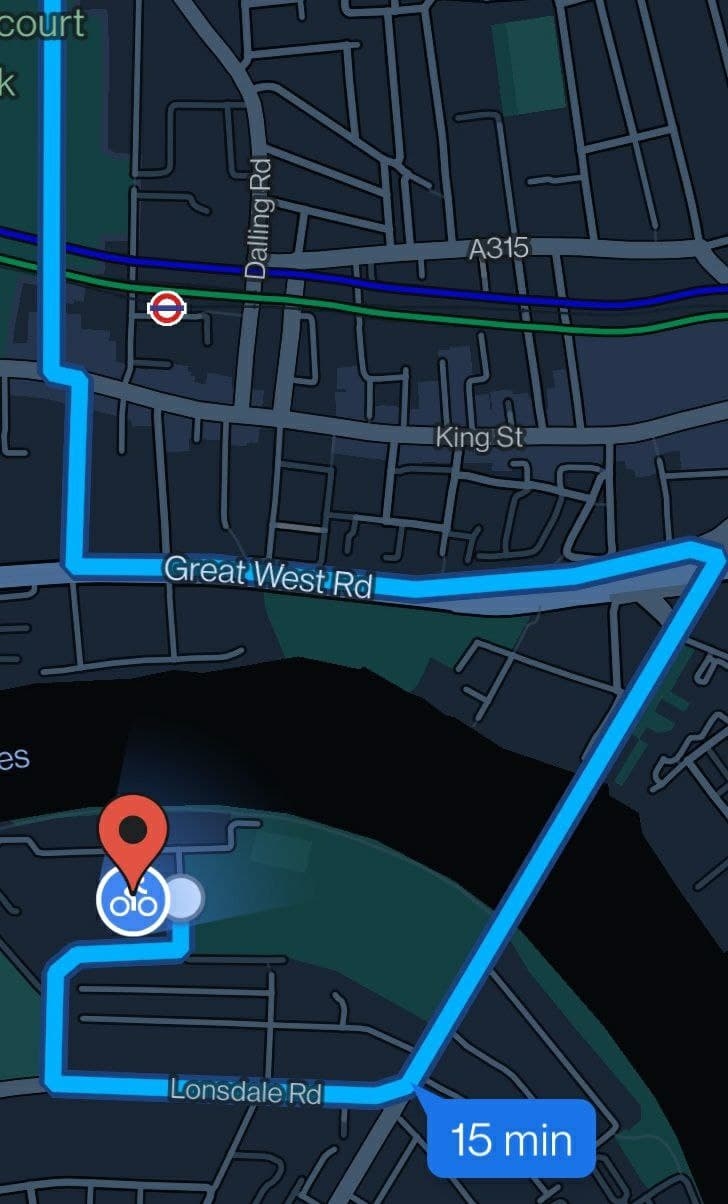
\includegraphics[height=5cm]{route.jpg}
    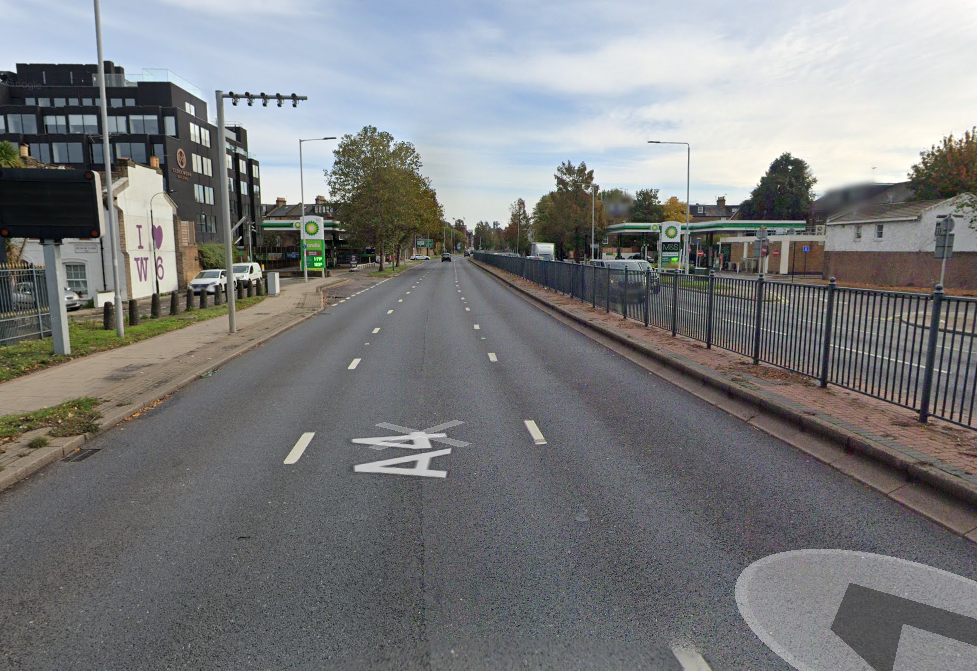
\includegraphics[height=5cm]{dangerous.png}
\end{center}
    \caption{Route suggested by google maps}
\label{route}
\end{figure}
Many of these route finding applications don't take into account safety considerations. This is shown in Figure \ref{route} which shows the route Google Maps suggests that I cycle to school by. The route includes the A4, which is a very dangerous stretch of road for cyclists as it is a 3 lane road. 
My plan is to use accident statistics to work out which roads are dangerous and then avoid them. This would be done by imposing a cost for going somewhere that there had been an accident.
\subsection{Client}
I interviewed Yuvraj Dubey, one of my classmates, to talk about whether they would be intererested in a product that attempted to calculate safe routes to cycle. 
\begin{center}
    Do you own a bicycle?\\
    \textit{Yes}\\
    Do you cycle regularly?\\
    \textit{Yes}\\
    Do you ever feel in danger while cycling?\\
    \textit{Yes}\\
    When do you feel in most danger while cycling?\\
    \textit{At a Junction near Victoria, where there is a right turn and no cycle lane to do it in. I attempted to go this way once and was almost hit by a bus. }  \\
    Are you aware of your surroundings while cycling?\\
    \textit{Not really}\\
    Do you feel aware of the places which to cycle in safely, does this change when you are in places you commonly go? \\
    \textit{No, but especially where I don't know where I am because then I do not know where it is safe to cycle. When I cycle home I have learnt a safe route, but if asked to cycle somewhere I did not know I would most likely end up in a dangerous place.} \\
    Would you use an application that tells you safe routes to get places?\\
    \textit{Yes}\\
    Would you be happy using a command line application for this?\\
    \textit{Yes}\\
    If said application took more than 60 seconds to calculate a route would you lose patience?\\
    \textit{Yes, probably}\\
    Have you found that cycling directions generated by current products are safe and efficient?\\
    \textit{They are definitely efficient, but they often take me onto busy roads and junctions which can be less safe.}
\end{center}
From this interview and my own experiences cycling in London I determined that there was an application for my idea, but only if it ran in a reasonable amount of time and was otherwise easy to use, as people struggle to find safe routes themselves, especially when going somewhere they had not previously been, and commercial
products such as Google Maps don't generate safe routes. 
\newpage
\subsection{Similar Systems}
\begin{figure}[h]
    \begin{center}
        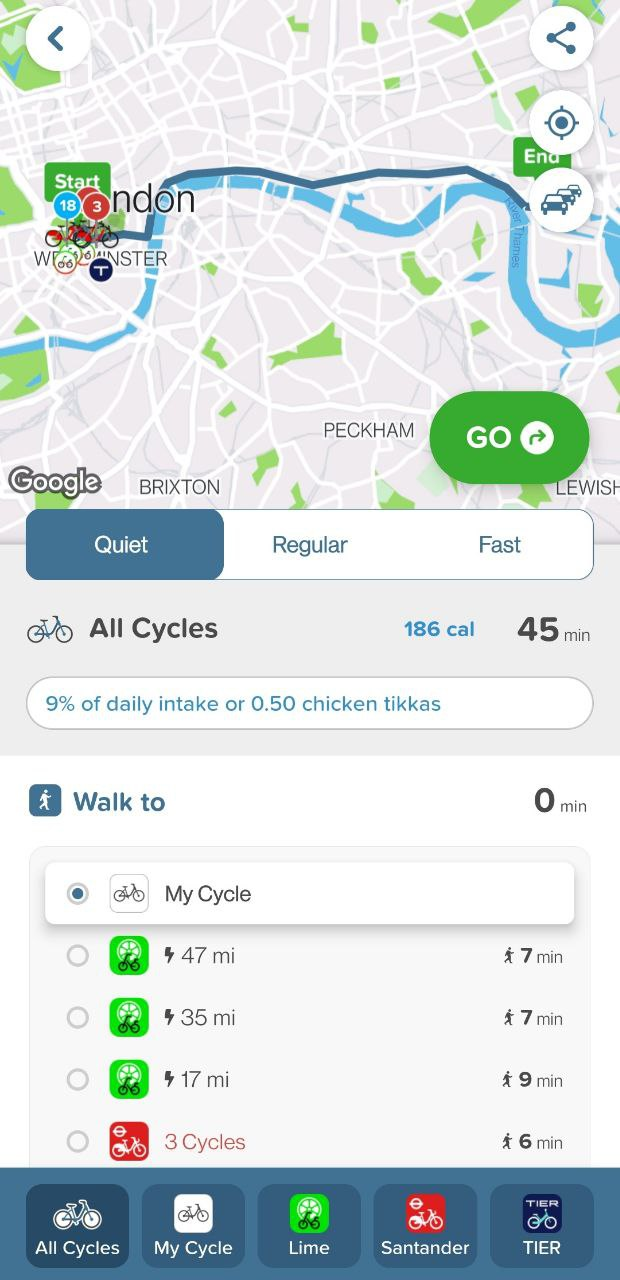
\includegraphics[height=10cm]{citymapper.png}
    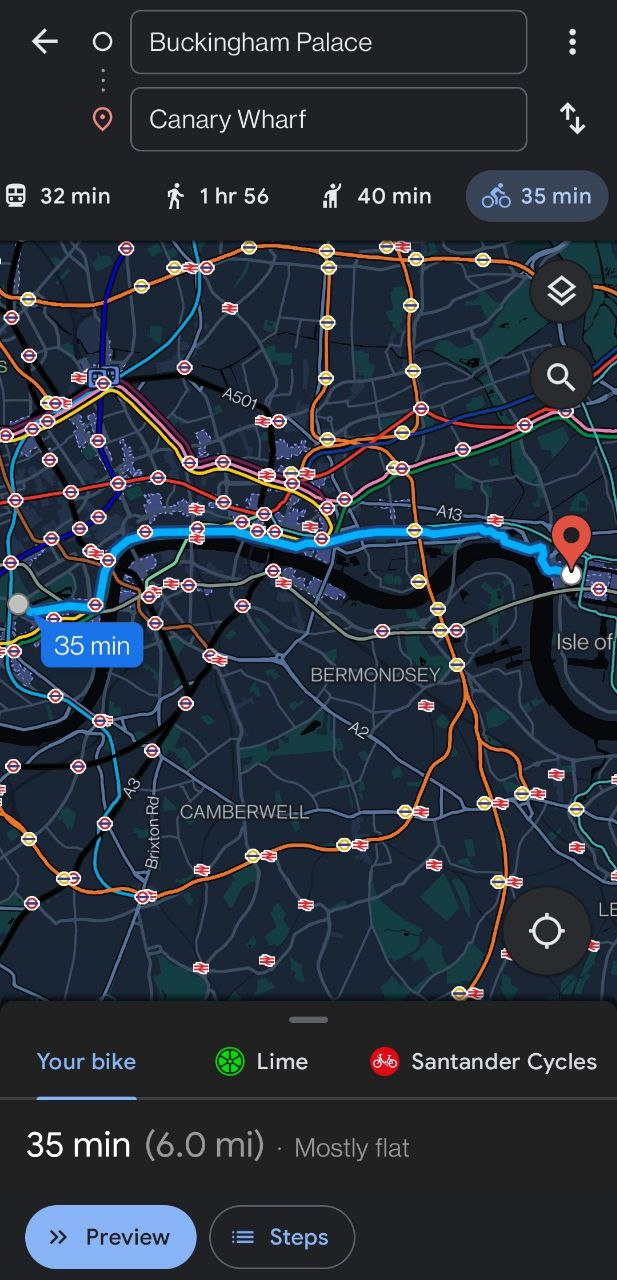
\includegraphics[height=10cm]{googlemaps.png}
\end{center}
    \caption{Citymapper and Google Maps respectively, generating the same directions}
    \label{alternatives}
\end{figure}
There exist similar systems for route finding such as Google Maps and Citymapper. These have advantage's over what I will be able to offer such as being able to use live traffic data, and having a good user interface. Citymapper has a option to choose between "Quiet", "Regular", and "Fast" routes, which seems to be based on the type of road you are taken down.
However they don't really take accident density into account which will be my aims.
\subsection{Features}
\subsubsection{Map data}
I need a data source which can provide data on roads that are legal to cycle on as well as being freely available for me to use. I settled on Open Street Map, a project which combines data gathered by volunteers into one massive freely available map. The map is downloadable in the form of a large XML file or PBF file. A PBF file is just a binary version of the same thing. I could write code to parse this myself, but instead I think that I am going to use the library libosmium
which works in C++.
\subsubsection{Accident Data}
\begin{figure}
    \begin{center}
        \begin{tikzpicture}[scale=1]
        \draw[gray, thick] (-4,0) -- (4,0);
        \draw[gray, thick] (0,-4) -- (0,4);
        \filldraw[black] (0,0) circle (2pt) node[anchor=west]{};
        \filldraw[black] (0,2) circle (2pt) node[anchor=west]{};
        \filldraw[black] (2,0) circle (2pt) node[anchor=west]{};
        \filldraw[black] (-2,0) circle (2pt) node[anchor=west]{};
        \filldraw[black] (0,-2) circle (2pt) node[anchor=west]{};
\filldraw[black] (0,-4) circle (2pt) node[anchor=west]{};
\filldraw[black] (0,4) circle (2pt) node[anchor=west]{};
\filldraw[black] (4,0) circle (2pt) node[anchor=west]{};
\filldraw[black] (-4,0) circle (2pt) node[anchor=west]{};
    \end{tikzpicture}
\end{center}
    \caption{Typical OSM representation of an intersection}
    \label{intersection}
\end{figure}
Transport for London has an excellent API which you can download accident data from. The data comes in JSON files and contains information about what type of vehicle was involved in each accident, the severity, and the coordinates of the accident. 
I need to find a way of mapping the coordinates onto the road network so that the danger of roads can be calculated as accurately as possible. Originally I was looking at adding the accident to the nearest edge in the graph but I decided against this after considering how intersections 
are typically represented in OSM. Road intersections typically look something like what is represented in Figure \ref{intersection}. If an accident were to occur at the intersection it would end up being added to one of the segments leading into the intersection, so the danger would not be properly calculated if not passing through that segment. Instead I thought about adding the danger to the nearest node, so that the accident would always be counted when a route passes through that intersection.
The other problem that I have to deal with, if adding data to the nearest node is that the density of nodes is not constant. Straighter roads will not need to use as many OSM nodes as curved roads, so i might incorrectly add cost to the wrong node. My proposed solution to this is to interpolate in nodes to a very high density to deal with this problem.
\subsubsection{Traffic Data}
The main problem with this is that the accident data is absolute and can thus not be used to calculate probabilities. For example, more accidents happen on King's Street than the dangerous road I showed earlier, but this doesn't mean that King's Street is more dangerous merely that more cyclists travel on it. This means that I need to get accurate cyclist traffic data for the whole of London in order to turn my accident statistics into accident probabilities.
The Department for Transport and the Office for National Statistics both keep data on traffic, but it isn't applicable because cycle data is only given as a total \footnote{0.6 billion miles per year in London} and at specific count points.
This means that I will either need to work out traffic data or get it from some dataset, such as Strava's Global Heatmap. \\
Luckily the rest of the application can work without including traffic data so my plan is to deal with this problem at a later time or hope that the avoidance of accidents alone will be enough.  
\subsubsection{Finding the shortest route}
Algorithms for finding the shortest path in a Graph are abundant. The most well known is Dijkstra's algorithm, and it's variant A*. In large Graphs, both Dijkstra's algorithm and A* can be very slow. I will most likely use preprocessing based algorithms such as ALT*/Contraction Hierachies to make my program run a lot faster.
This preprocessing will take a long time, but when completed it will significantly reduce the time taken to complete searches. 
\subsubsection{Class Layout}
Insert class layout and associated planning here.
\subsection{Critical Path}
\begin{itemize} 
    \item Download accidents from the TFL API, parse for accidents that are of interest, and store it in a format that can be easily parsed later
    \item Import OSM map of London as a Graph which can be easily queried.
    \item Write code that imports the accident data and connects it to given Graph nodes.
    \item Write a simple Dijkstra's Algorithm method of finding the shortest path.
    \item Write a preprocessing based method of finding the shortest path.
    \item Write a frontend for inputing data about the route. 
\end{itemize}
\newpage
\subsection{Specification}
\begin{enumerate}
\item Accident Download System
\begin{enumerate}
    \item The System must be capable of interfacing with the TFL API to download accidents
    \item The System must be capable of parsing accident data to determine which accidents are relevant
    \item The System must be capable of storing accident data in a easily accessible file for the route finding algorithm to parse
\end{enumerate} 
\item Route Finding System
\begin{enumerate}
    \item  The System should be capable of processing an Open Street Map map file into a suitable data structure
    \item The System should be capable of processing the accident data from the Accident Download System
    \item The System should be capable of attaching the data from the Accident Download System to the Suitable Data Structure from specification point \textbf{2.1}
    \item The System should be capable of using Accident Data combined with other suitable cost estimation functions to find a directed route between two points that are places on roads in London
    \item The System should always suggest a route that can be followed while observing all currently known laws of physics
    \item The System should always suggest a route that can be followed while observing all international, national, local laws and all releveant bylaws
    \item The System should suggest a safe route wherever possible
    \item The System should have guards in place for certain types of roads which are deemed too dangerous to consider
    \item The System should be able to generate this route quickly
    \item The System should have a mode for preprocessing to make the route generation even quicker
    \item When using the same parameters, the route generated using a preprocessed graph and associated algorithms should be the same as that generated by the non-preprocessing based approach
    \item The System should be easy to use
    \item The System should not crash, and should give appropriate non crashing errors if user data is determined to be bad
    \item The parameters for the cost estimation functions should be user definable, but sensible defaults should also be defined
\end{enumerate}
\end{enumerate}
\newpage
\section{Design}
\subsection{Accident Download System}
As outlined in the Specification, this system should be capable of interfacing with the TFL API, downloading the accidents, deciding which ones are relevant, and storing this in a useful format.
\subsubsection{Pulling from the TFL API}
The Transport For London API is an excellent API which can provide information on many different aspects of the Transport For London network. The specific API which I used is the AccidentStats API.
This API is very simple, you simply request a given year and a JSON object is returned which contains all of the accidents that happened in london that year. These consist of all the accidents that were reported tocdepth
the police as happening in that year. Of course, there will be many more accidents than are on the API, but these will mostly be more minor accidents.
The Data is returned as a list of accidents, formatted as shown in Figure \ref{Default}.
\begin{figure}[t]
\begin{lstlisting}[language=Python]
[{
    "id": 0,
    "lat": 0.0,
    "lon": 0.0,
    "location": "string",
    "date": "string",
    "severity": "string",
    "borough": "string",
    "casualties": [{
        "age": 0,
        "class": "string",
        "severity": "string",
        "mode": "string",
        "ageBand": "string"
    }],
    "vehicles": [{
        "type": "string"
    }]
}]
    \end{lstlisting}
\caption{The Default output from the API}
\label{Default}
\end{figure}
\\
As the data about accidents that happened in the past is not going to change any time soon, and TFL only updates this API every year, it is simplest just to download the files once, parse it once, and then 
use that result in the route finder.\\
TFL started gathering this data in 2005, and the most recent update was in 2019, so I wrote a simple python script to download all the data from 2005 to 2019 and save it in a subfolder called \texttt{accidents}.
The program loops through all the years between 2005 and 2019 and fills a JSON file for that year. \\
\subsubsection{Parsing the Data}
The next step was to go through the data from all the years, and save all the accidents that were pertinent to my project. As seen in Figure \ref{Default}, each accident listing has information on casualties,\\
of which there may be many. As this is a cycling application, I only wanted data on accidents where at least one of the casualties was a cyclist. The API provides a lot of data, but all that I decided was relevant was
the latitude and longitude, as well as the severity of the incident. All of this data was ultimately saved to a file called \texttt{output.json}.
 The code used for parsing is shown in Figure \ref{Download.py}.
\begin{figure}[t]
    \begin{lstlisting}[language=Python]
import json
accidents = []
for year in range(2005,2020):
    print(len(accidents), year)
    with open(f"accidents/{year}.json","r") as outfile:
        data = json.load(outfile)
    for x in data:
        if len([person for person in x["casualties"] if person["mode"] == "PedalCycle"]) >= 1:
            accidents.append([x["lat"],x["lon"],x["severity"]])
with open("output.json","w") as outfile:
    json.dump(accidents,outfile)
    \end{lstlisting}
\caption{The script I wrote to parse the data}
\label{Download.py}
\end{figure}
\label{end}
\newpage
\subsection{Route Finding System}
\subsubsection{Overview and Design Choices}
I decided to use Kotlin for this project. Kotlin is related to Java in that it allows access to all the Standard Java Libraries, as well
as external ones, and it runs in the Java Virtual Machine. Kotlin does not need to maintain backwards compatability with old Java code,
so it has a much cleaner API and has nice syntax. As this was a new project not dependent on using Java code Kotlin was an obvious choice. 
Furthermore, Java code can be easily translated into Kotlin code, so I could code things in Java then translate over if necessary.\\
As seen in Figure \textcolor{red}{[insert figure here]}, I decided to define 3 main classes for my NEA. \texttt{OpenStreetMap} contains methods for parsing OSM files and creating a graph.
\texttt{OpenStreetMap} contains a single instance of the \texttt{GeographicGraph} class by object composition. This is because there will only be one \texttt{GeographicGraph}
class associated with a given OSM file, and this system could be easily extended to hold information on two separate graph areas at the same time, which could be used if I wanted
to extend the system to more cities. The \texttt{GeographicGraph} can contain an instance of the \texttt{ContractableGraph} class, if it has been contracted. If it has not been contracted,
this class will not exist.\\
I also created two other classes, \texttt{IntTuple} and \texttt{DoubleTuple}, which are used in priority queues in both the \texttt{GeographicGraph} and \texttt{ContractableGraph} classes.
\subsubsection{Open Street Map Data}
Open Street Map is a world map generated by user mapping. It contains multitudes of data on all sorts of mappable things, from the height of stories to the roads that encompass them.

\end{document}